\documentclass[12pt]{article}
\title{Maximal point problem}
\author{林橋毅 111502563}
\usepackage[UTF8]{ctex}
\usepackage{graphicx} %插入图片的宏包
\usepackage{float} %设置图片浮动位置的宏包
\usepackage{caption}
\usepackage{subfigure} %插入多图时用子图显示的宏包
\usepackage{algorithm}
\usepackage{algpseudocode}
\usepackage{amsmath}
\usepackage{graphics}
\usepackage{epsfig}
\usepackage{amssymb}
\usepackage{bm}
\newtheorem{definition}{Definition}

\begin{document}
\captionsetup[figure]{labelfont={bf}, labelformat={default}, labelsep=period,name={Fig.}}
\maketitle

\part{Introduction}
在最大點(Maximal point)問題中是:找出點集合 S 中不被集合中任一一點支配的點,如果在點集合 S 中的兩個點 p 和 q,若 q 的每個維度的值皆大於等於 p 在該維度的值,我們則稱 q dominates p(q 支配 p)。\\

本篇基於二維最大點演算法的基礎上,使用分治的方法優化並實作出比暴力求解更有效率的三維最大點演算法,該演算法的時間複雜度在測資隨機時為線性時間複雜度。

\begin{definition}
	Point \textbf{p} \textbf{dominates} point \textbf{q} if $x_i(p)$ >= $x_i(p)$ for i = 1,2,...d. (通常在 d <= 3 的情況下令 $x_1$, $x_2$, $x_3$ 分別為 x, y, z)
\end{definition}

\begin{definition}
In a finite set of point S, point p $\in$ S is a \textbf{maximal point} if there does not exist a point q $\in$ S such that q \textbf{dominates} p.
\end{definition}


\part{Method}

\section{Two dimensionl}
求解二維最大點問題可以用以下掃描線的技巧求解,這個演算法可以分為以下步驟:
\begin{itemize}
	\item 將點以 x 座標由大到小排序
	\item 隨著 x 由大到小遍歷所有點並紀錄目前最大 y 座標,若遇到一點之 y 座標比目前紀錄最大值還大則此點是一個 Maximal point,將其輸出並更新最大的 y 座標。
\end{itemize}

\begin{algorithm}[H]
	\caption{Pseudocode}
	\begin{algorithmic}
		\State sort point by x-corrdinate //將所有點依照 x 座標由大到小排序好
		\State maxY = $p_0$ - 1
		\For{$i=0$ to $n$}
			\If{$p_i$ > maxY}
				\State M* $\leftarrow$ $p_i$
				\State maxY = $p_i$
			\EndIf
		\EndFor
	\end{algorithmic}
\end{algorithm}

\section{Three dimension}

\subsection{Brute force solution}
暴力求解法是直接對於點集合 S 的用兩兩比較的方式,檢查每一個點是否被任何一點 dominates,如果沒有任何點可以支配他則此點為一個 Maximal point。

\begin{algorithm}[H]
	\caption{Pseudocode}
	\begin{algorithmic}
		\State M* $\leftarrow$ $\varnothing$	// M* 用來儲存找到的 Maximal point
		\For{$i=0$ to $N$}
			\State flag = True
			\For{$j=0$ to $n$, i $\neq$ j}
				\If{point $p_j$ dominates point $p_i$}
					\State flag = True
				\EndIf
			\EndFor
			\If{flag == True}
				\State M* $\leftarrow$ $p_i$ // $p_i$ is a maximal point.
			\EndIf
		\EndFor
		\State sort(M*) //根據題目要求將 M* 排序好 
	\end{algorithmic}
\end{algorithm}

\subsection{Pruning solution}
觀察 3.1 的暴力求解法,我們可以觀察到,所有點無論如何都會被比較 N-1 次,但換個想法可以從紀錄有一點 $p$ 沒有可能是最大點,如果這個點 $p$ 不可能成為最大點時我們就可以直接跳過他,因為如果他不可能成為最大點代表我們找到一個點 $q$ 可以 dominates $p$,哪麼所有 $p$ 可以支配的點 $q$ 也都可以支配,所以如果能夠確定 $p$ 不為最大點便可以將其標記起來,後續比較時可以直接跳過以加速比較過程,經過實驗相較於暴力求解確實在執行時間有提升。

\begin{algorithm}[H]
	\caption{Pseudocode}
	\begin{algorithmic}
		\State M* $\leftarrow \varnothing$, check = {0}// M* 存最大點、check[i] 紀錄 $p_i$ 是否不可能為最大點
		\For{$i=0$ to $N$}
			\For{$j=0$ to $N$, i $\neq$ j and c[i] == 0}
					\If{$p_i$ dominates $p_j$}
				\State c[i] = 1
				\EndIf
			\EndFor
		\EndFor
		\State M* $\leftarrow p_i$ for check[i] == 0
		\State sort(M*)
	\end{algorithmic}
\end{algorithm}

\subsection{Divide and conquer method}
基於二維的求解,可以將有序的三維點切分成許多個二維的平面,分別求解每個平面再將每個平面的結果合併起來。紀錄每個平面的最大點集 $M_i$,接著隨著座標由大到小維護一個做為答案的最大點集 M*,依序遍歷每個點 p,如果不存在任何點 $q \in M*$ 使得 q dominates p,就將 p 放入 M*,這個演算法的時間複雜度為 $O(NlogN)$ 是線性時間複雜度。


\begin{definition}
	Finite set of point S, point p $\prec$ S if $\neg \exists$ point q $\in S$ such that q dominates p.
\end{definition}

\begin{algorithm}[H]
	\caption{Pseudocode}
	\begin{algorithmic}
		\State M $\leftarrow \varnothing$, M* $\leftarrow \varnothing$ // M 存每個平面的最大點、M* 為答案的最大點集合
		\State sort(p) // 將點排序好(x 由大到小若相等則 y 由大到小,依此類推...)
		\State Zmax = $p_0$ - 1 
		\For{$i=0$ to  $N$}
			\If{i $\neq$ 0 and $p_i.x$ != $p_{i-1}.x$}
				\State Zmax = $p_i.x -1$
			\EndIf
			\If{$p_i.z$ > Zmax}
				\State Zmax = $p_i.z$
				\State M $\leftarrow p_i$
			\EndIf
		\EndFor
		\For{$i=0$ to $M.size$}
			\If{$\neg (p_i \prec M*)$}
				\State $M* \leftarrow p_i$
			\EndIf
		\EndFor
	\end{algorithmic}
\end{algorithm}
\part{Experimental result}
我使用 generator.cpp 產生點座標範圍為 0 到 100000 的隨機測資,測試從 N = 1 到 N = 20000 的時間表現,可以看到不管是剪枝法還是分治法都相對於暴力求解有優秀的效能提升,尤其是分治法為線性時間複雜度。

\begin{figure}[H]
	\centering
	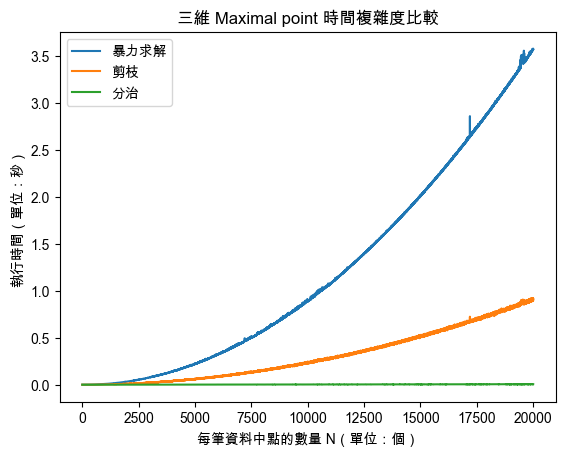
\includegraphics[width=0.7\textwidth]{time_compare}
	\caption{演算法時間複雜度比較圖} %最终文档中希望显示的图片标题
	\label{Fig.main2} %用于文内引用的标签
\end{figure}

\part{Conclusion}

\end{document}